\begin{frame} \frametitle{\vspace*{0.5cm}Results: Late-time evolution of the interface}
  \begin{figure}
    \centering%
    \only<1>{
      % \begin{tikzpicture}
      %   \node[anchor=south west,inner sep=0] (image) at (0,0) {
      %   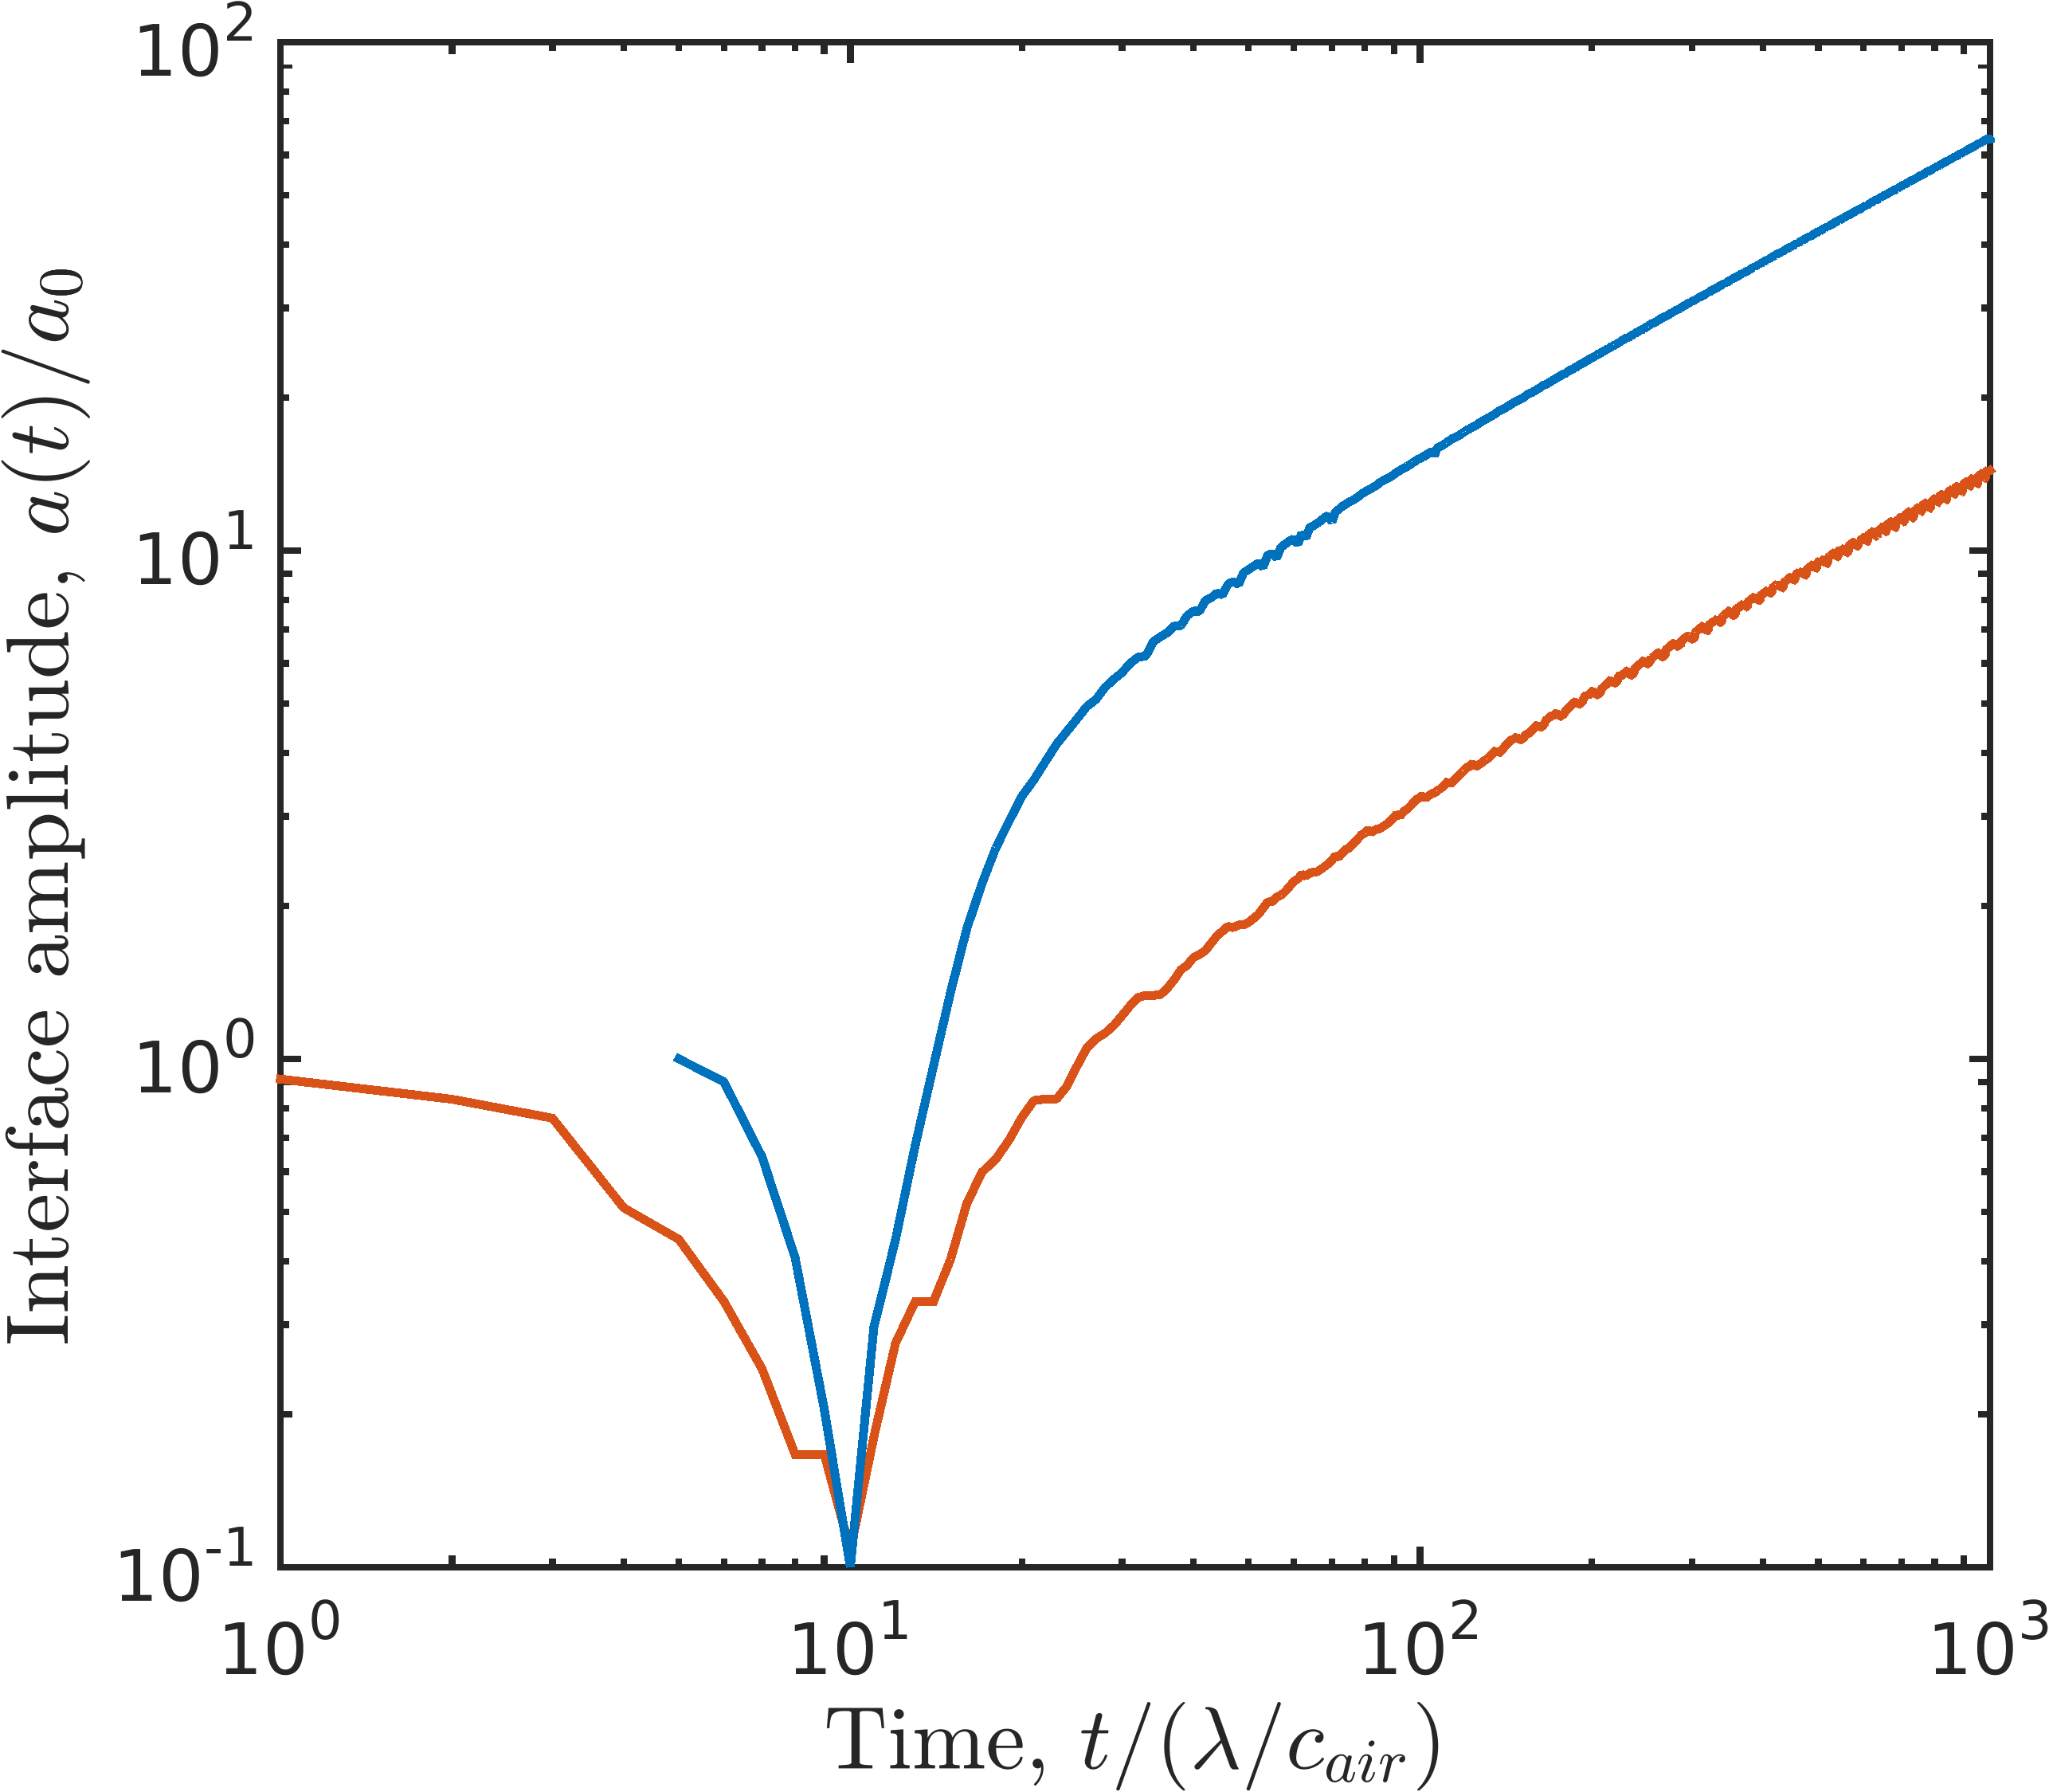
\includegraphics[width=0.6\textwidth]{../figs/lung_figs/interface_multi-amp_loglog_roe_t1000_nolines}
      % };
      %   \begin{scope}[x={(image.south east)},y={(image.north west)}]
      %     \node[font=\footnotesize,right] at (0.4,0.7){ $10$ MPa};
      %     \node[font=\footnotesize,right] at (0.6,0.4){ $5$ MPa};
      %   \end{scope} 
      % \end{tikzpicture}
    }
    \begin{tikzpicture}%
      \node[anchor=south west,inner sep=0] (image) at (0,0) {%
        \only<1>{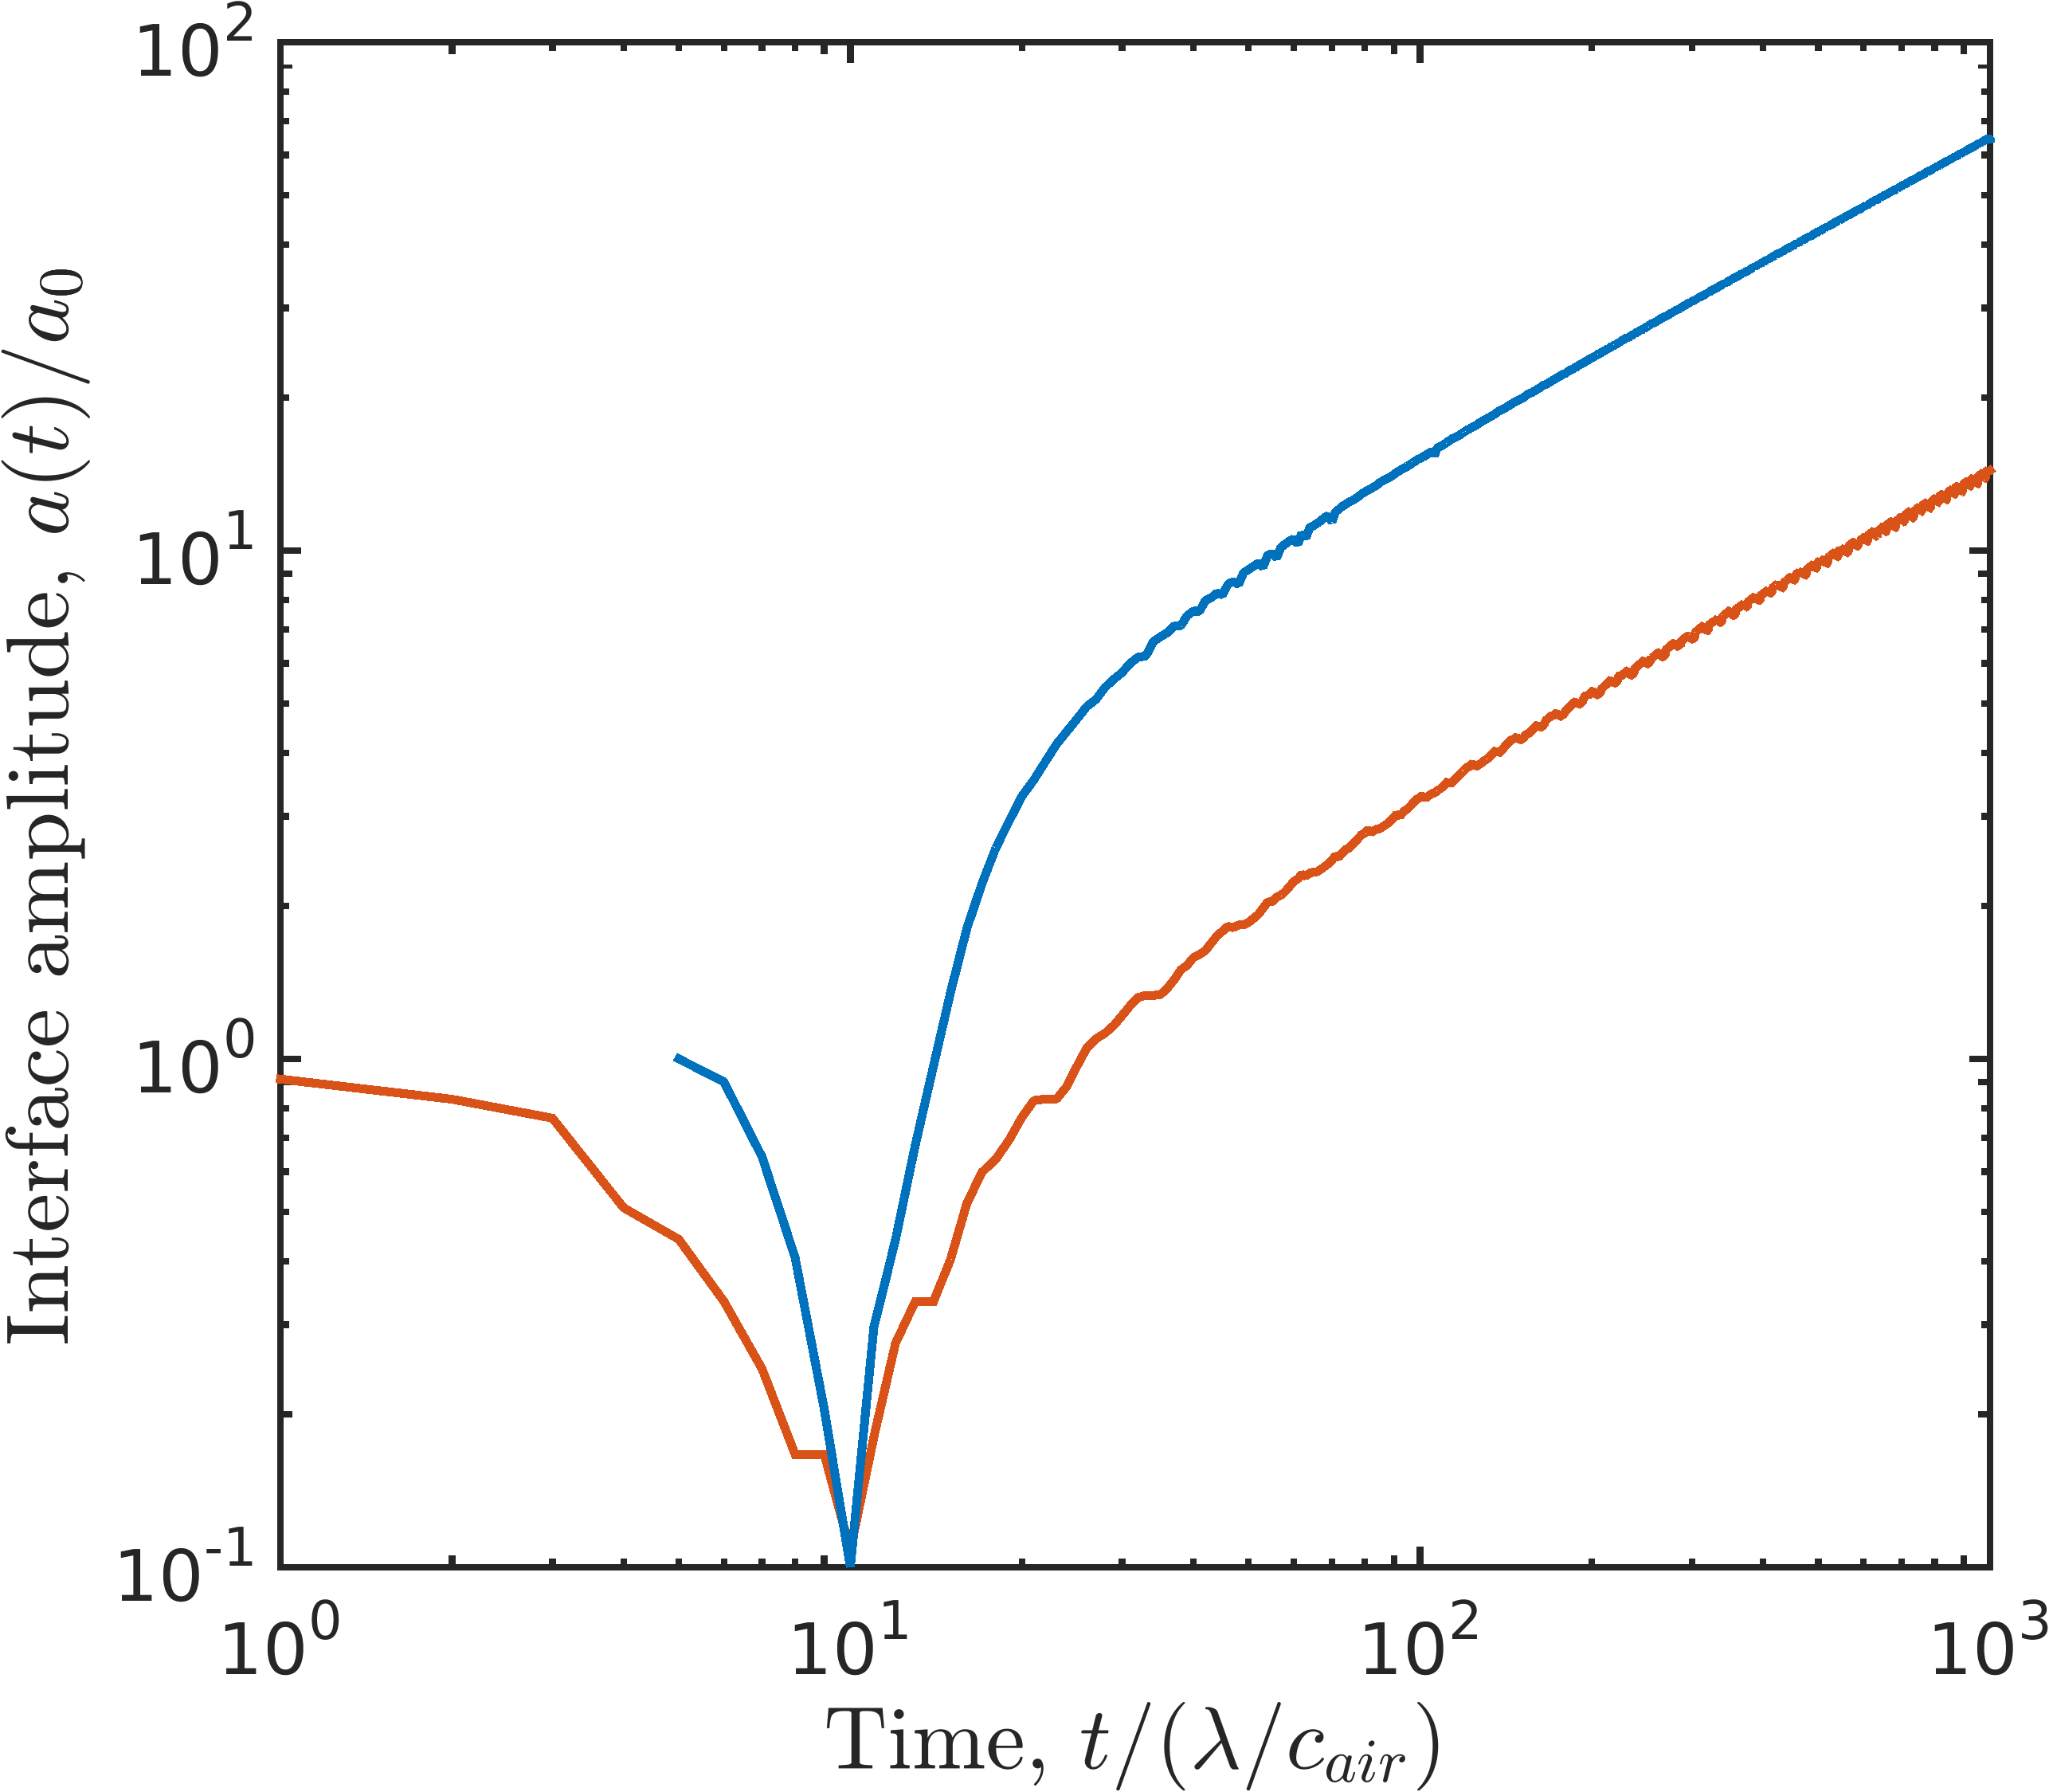
\includegraphics[height=0.54\textheight]{../figs/lung_figs/interface_multi-amp_loglog_roe_t1000_nolines}}%
        \only<2->{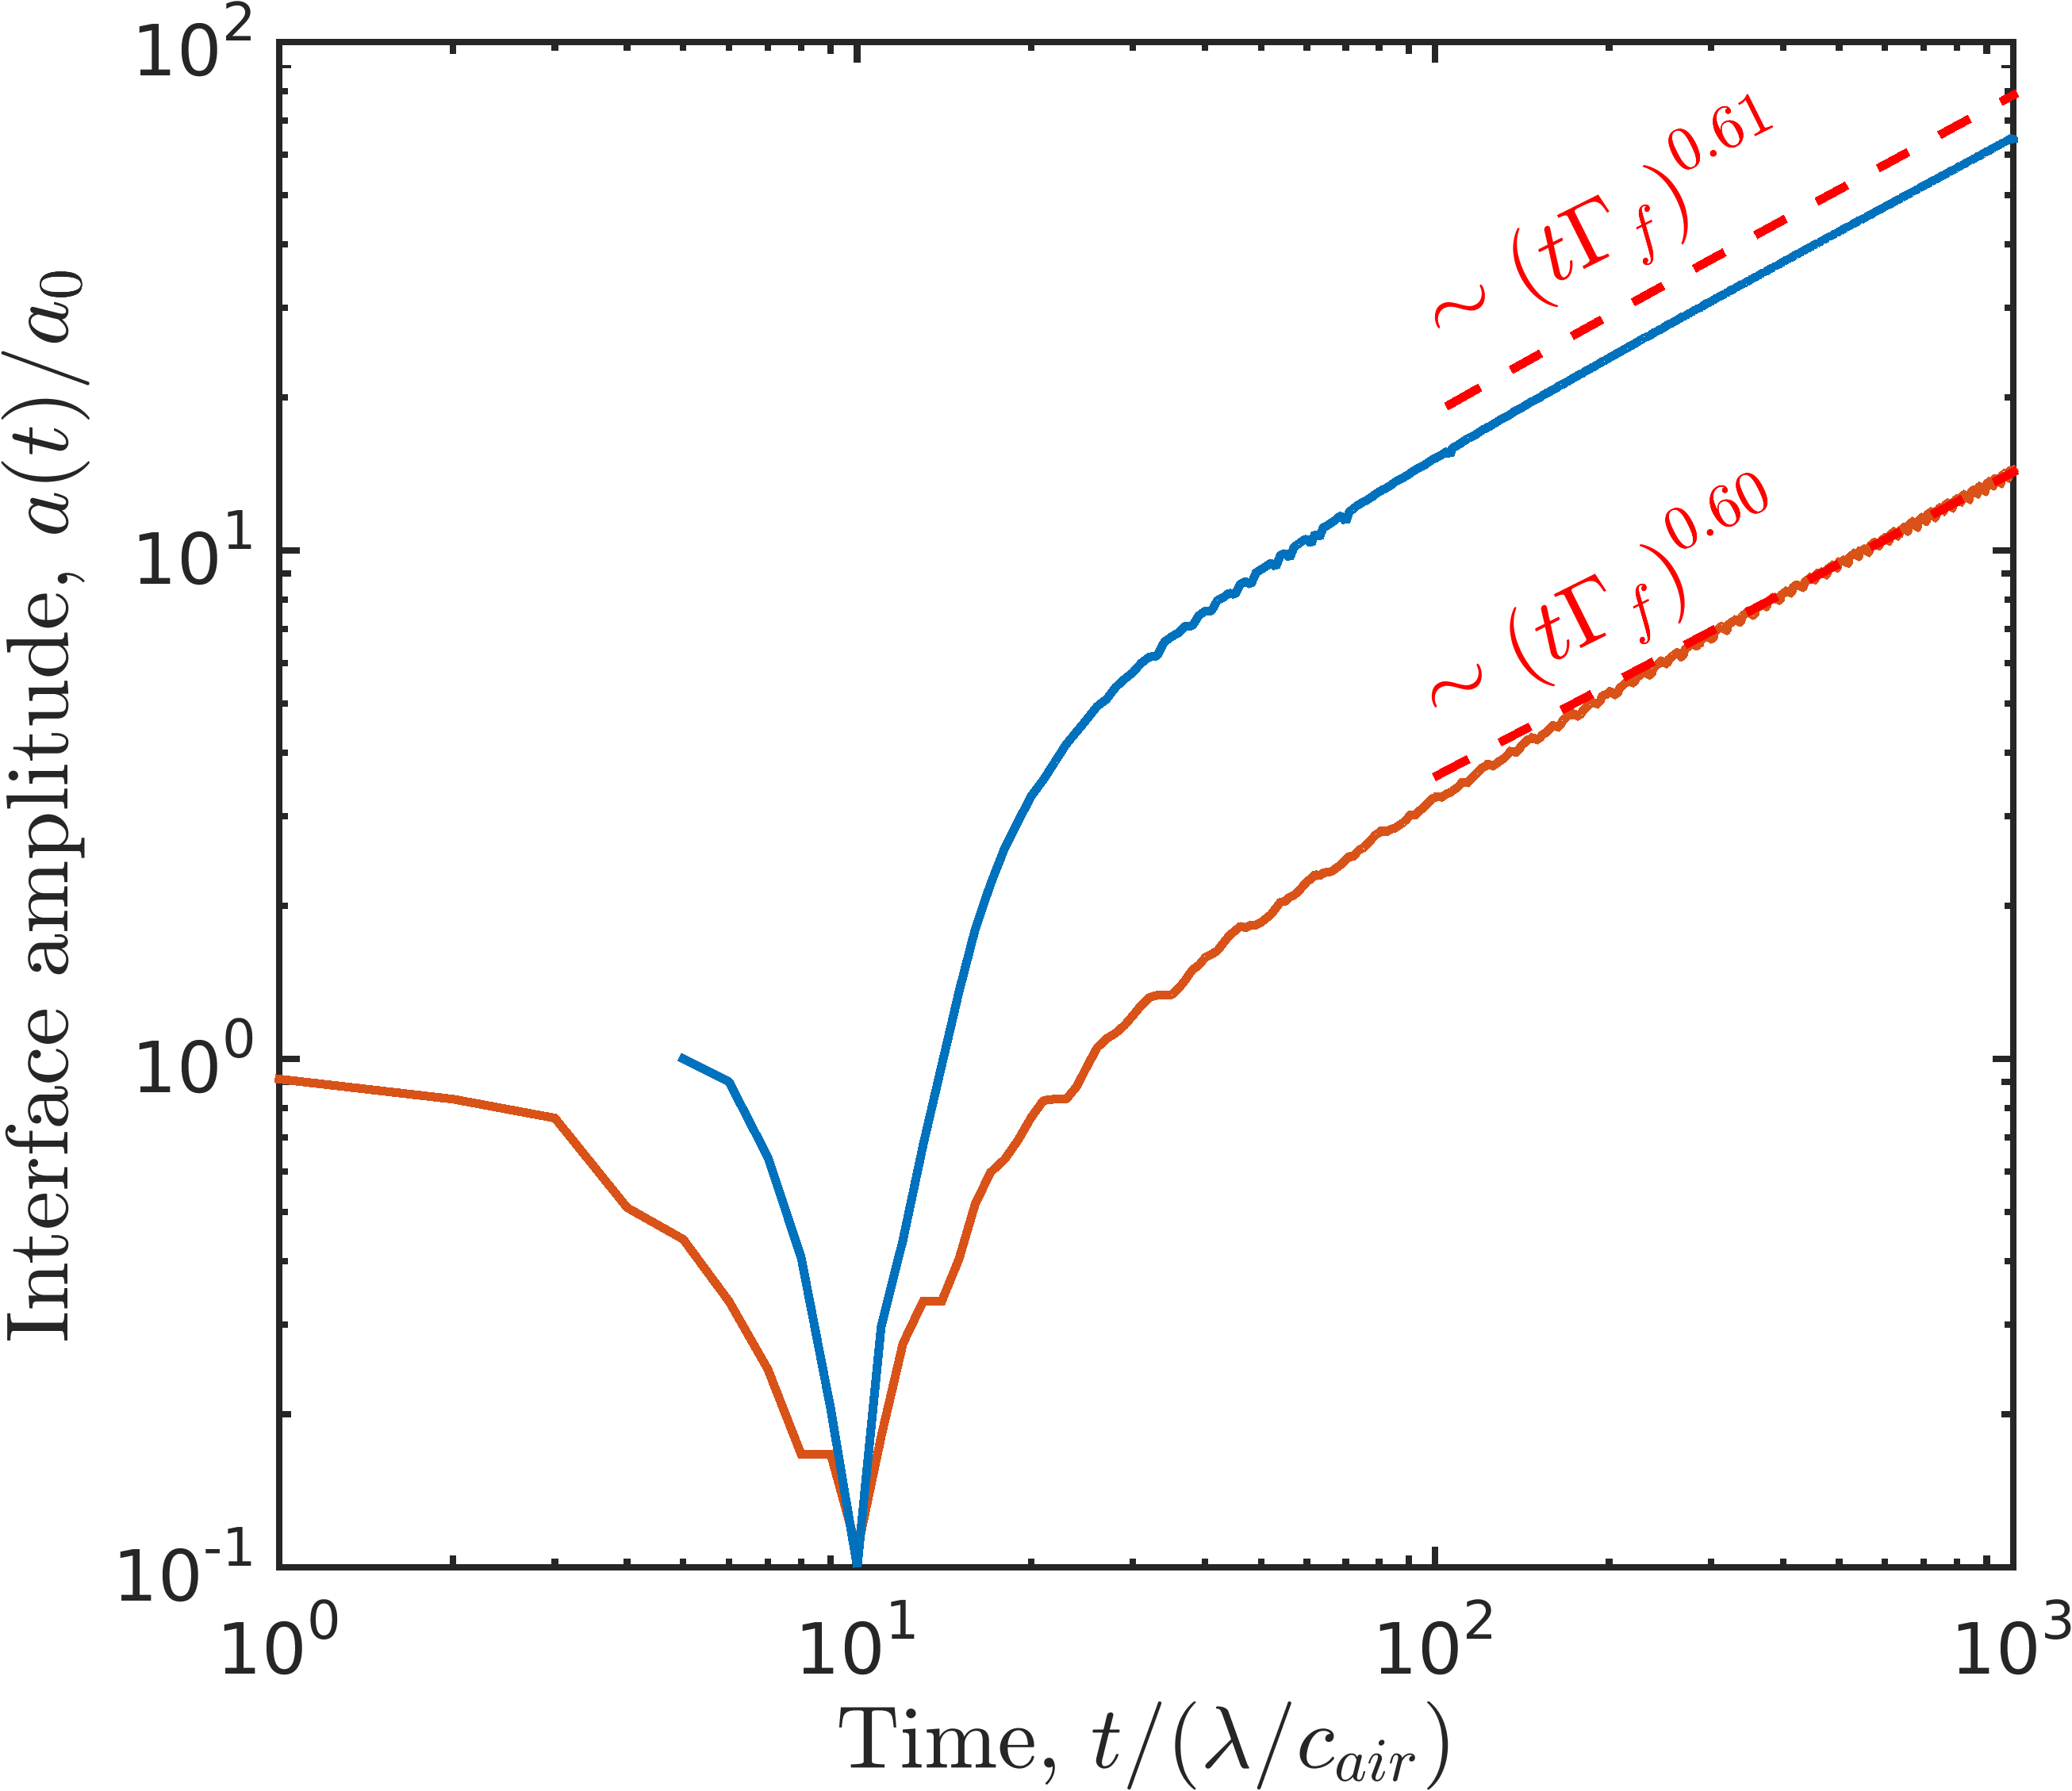
\includegraphics[height=0.54\textheight]{../figs/lung_figs/interface_multi-amp_loglog_roe_t1000}}%
      };%
      \begin{scope}[x={(image.south east)},y={(image.north west)}]%
        \node[font=\footnotesize,right] at (0.38,0.7){ $10$ MPa};%
        \node[font=\footnotesize,right] at (0.57,0.4){ $5$ MPa};%
      \end{scope}%  
    \end{tikzpicture}%
    \hfill%
    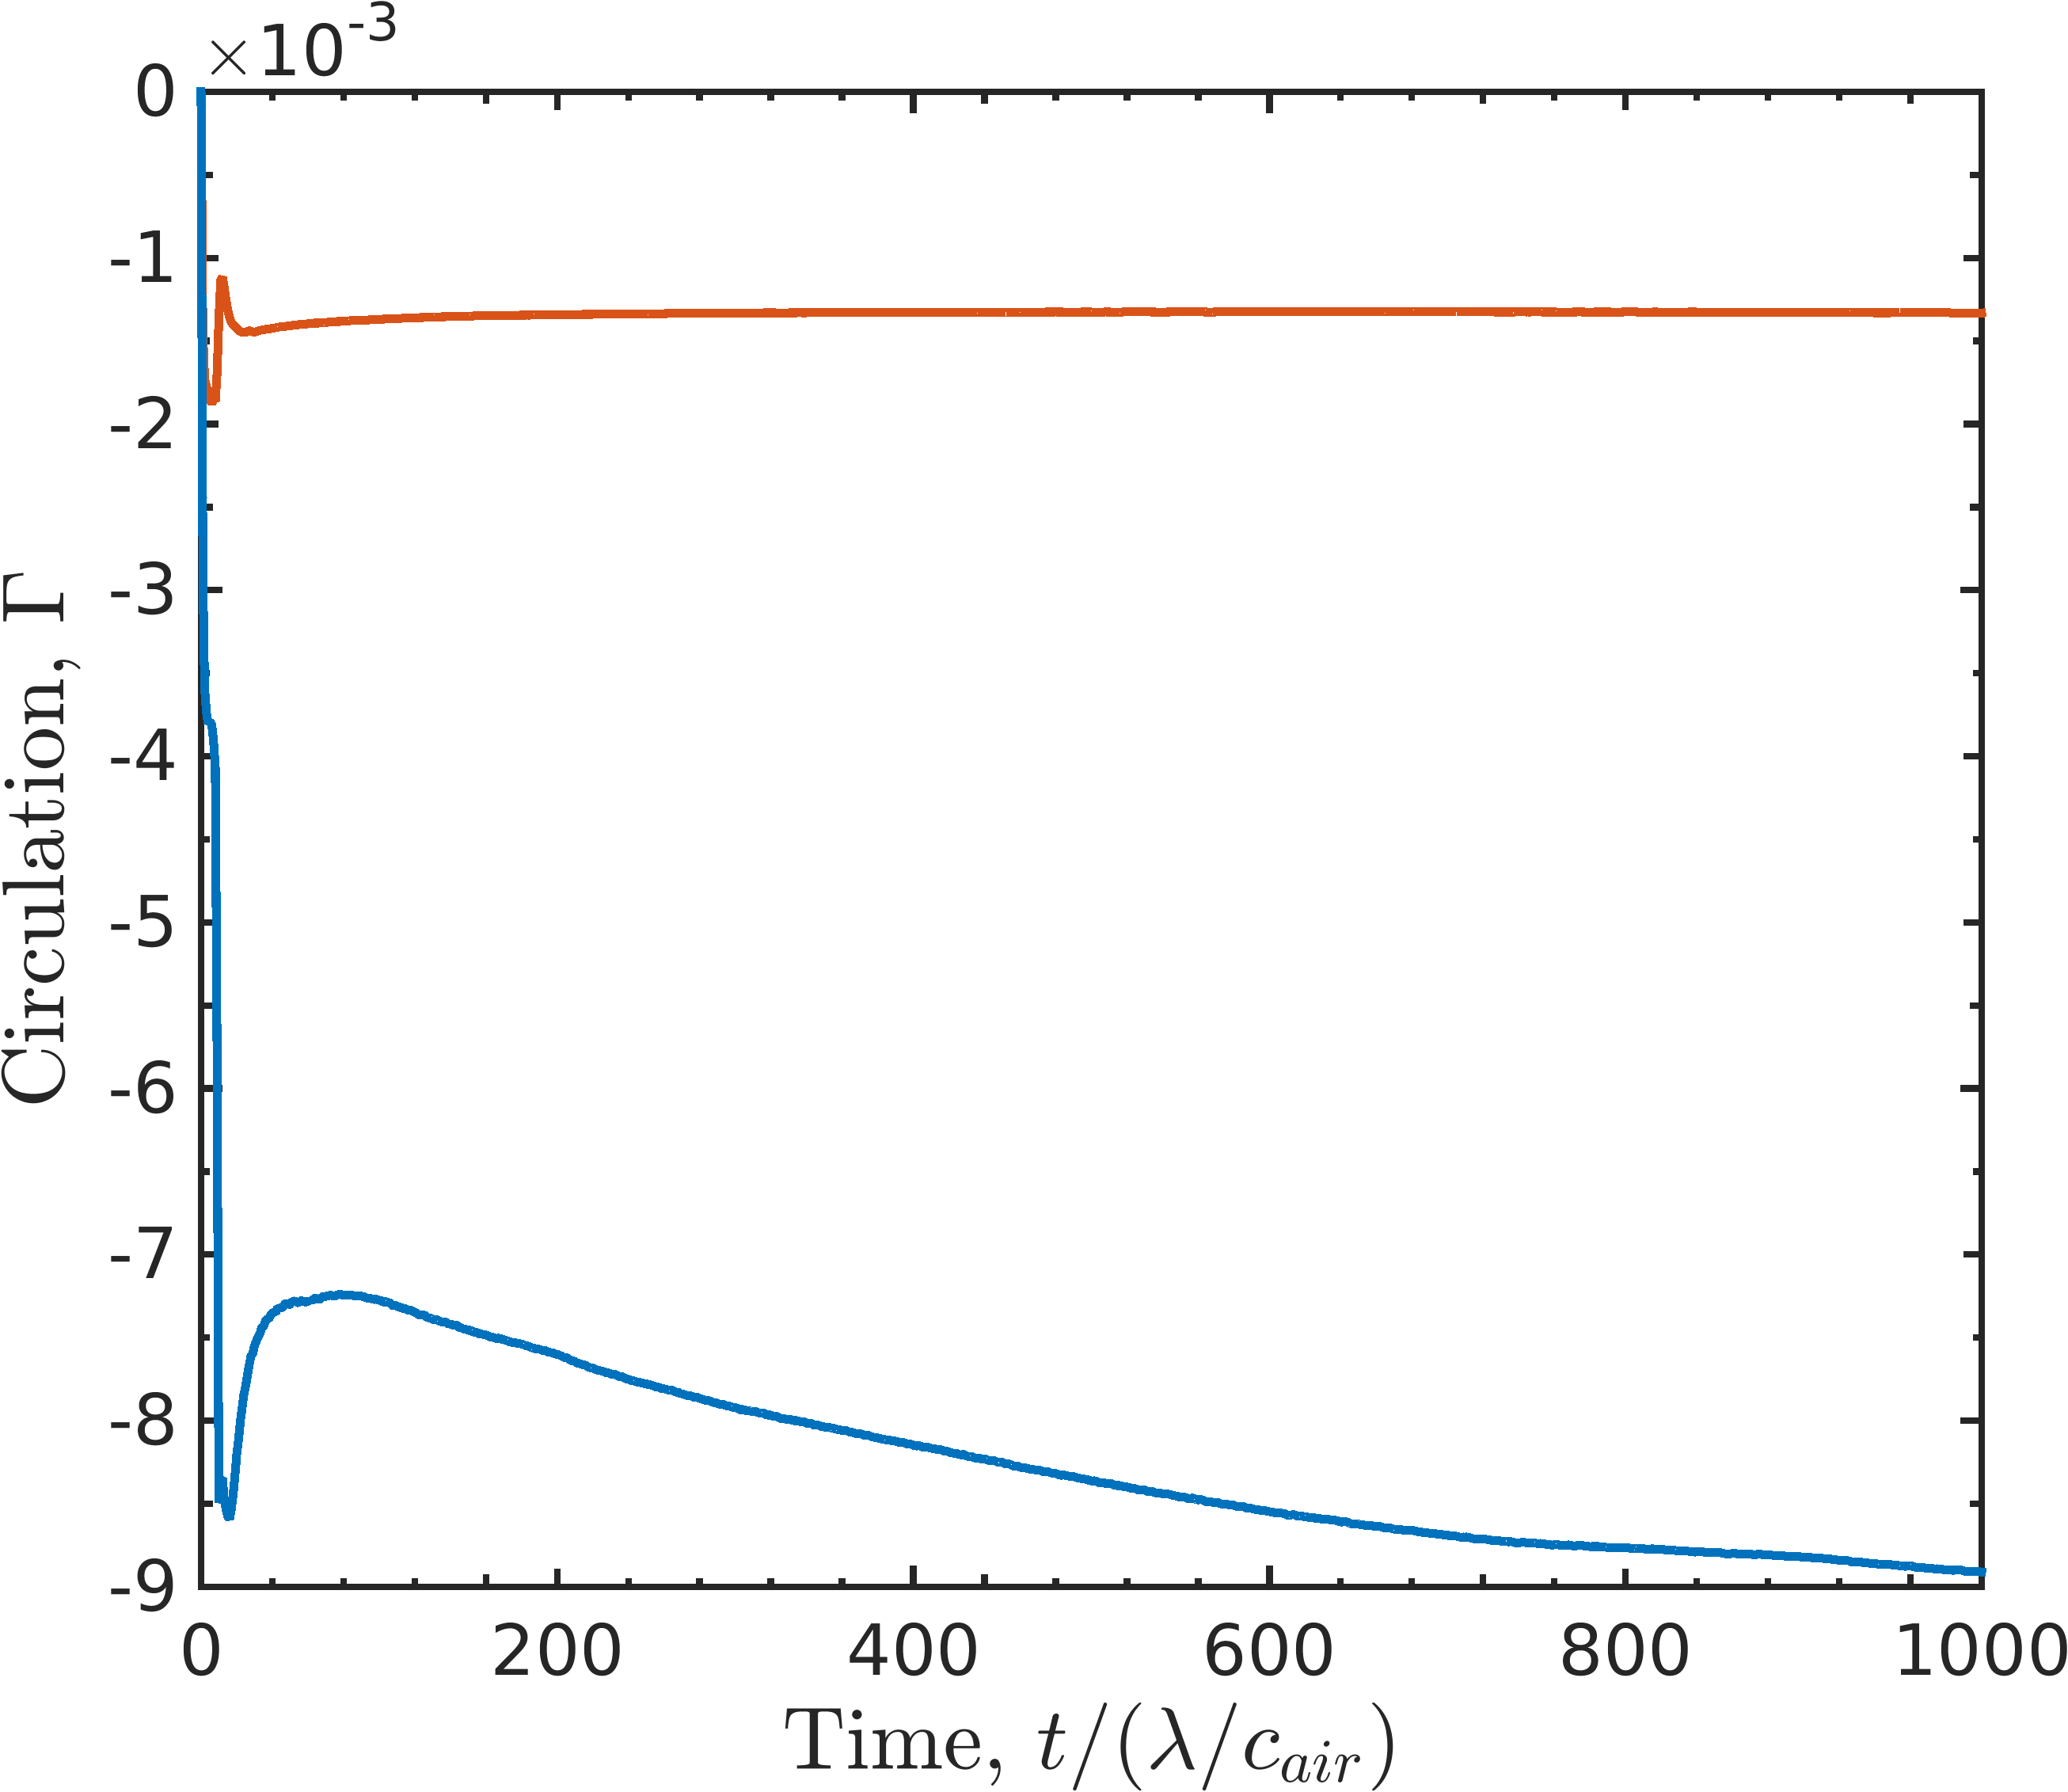
\includegraphics[height=0.54\textheight]{../figs/lung_figs/circulation_multi-amp_roe_t1000}%
  \end{figure}
  {\small
    From dimensional analysis, we expect a purely circulation growth of the interface perturbation to behave according to $a(t) \sim \sqrt{\Gamma t}.$
  }
  \note{
    {\scriptsize
      \begin{enumerate}
      \item If we again look at our interface amplitude, now in the context of circulation.
      \item we expect from dimensional analysis that a purely circulation driven interface may grow as square root of time.
      \item Our actual results grow as $t^{0.6}$ based on the slope of a log-log plot. 
      \item This isn't quite correct, but part of the reason for this could be that there are multiple length scales in this problem, so the scaling may not be clean.
      \item Also, the vorticity is smeared around the domain by
        numerical diffusion, so not all of it is along the interface to
        drive the growth. But if this was the only problem, then the
        problem could be fixed by increasing resolution, which doesn't
        seem to be case for the resolutions that we can practically run.
      \item In any case, this is close and we expect that it explains most of what is happening here.
      \end{enumerate}
    }
  }
\end{frame}
%%% Local Variables:
%%% mode: latex
%%% TeX-master: "../main"
%%% End:
